\documentclass{article}
\usepackage{amsmath}
\usepackage{graphicx}
\usepackage{listings}

\begin{document}

\title{Lab Report: Bresenham's Line Drawing Algorithm}
\author{}
\date{}
\maketitle

\section*{PROBLEM STATEMENT}
To implement Bresenham's Line Drawing Algorithm in C using OpenGL, and to draw a line between two points on a 2D plane. The program will also draw the coordinate axes to visualize the line in the context of a Cartesian coordinate system.

\section*{THEORY}
Bresenham's Line Drawing Algorithm is an efficient way to generate points of a line between two given points in a raster display. It uses only integer addition, subtraction, and bit shifting, which makes it faster than other methods like the DDA (Digital Differential Analyzer) algorithm. The algorithm determines the points of an n-dimensional raster that should be selected to form a close approximation to a straight line between two points.

The key idea is to keep track of the error term, which is the difference between the actual and the ideal y-coordinate values. By incrementally updating this error term and the x and y coordinates, the algorithm plots the line pixel by pixel.

\section*{ALGORITHM}
\begin{enumerate}
    \item \textbf{Initialize}:
    \begin{itemize}
        \item Start with the initial point $(x_0, y_0)$.
        \item Calculate the differences: $\text{dx} = |\text{x1} - \text{x0}|$ and $\text{dy} = |\text{y1} - \text{y0}|$.
        \item Determine the step direction for x and y: $\text{sx} = \text{x0} < \text{x1} ? 1 : -1$ and $\text{sy} = \text{y0} < \text{y1} ? 1 : -1$.
        \item Initialize the error term: $\text{err} = \text{dx} - \text{dy}$.
    \end{itemize}
    \item \textbf{Plotting}:
    \begin{itemize}
        \item While the current point is not the end point:
        \begin{itemize}
            \item Plot the current point.
            \item Calculate the error term for the next point.
            \item Update the coordinates based on the error term.
        \end{itemize}
    \end{itemize}
    \item \textbf{Termination}:
    \begin{itemize}
        \item The loop terminates when the current point reaches the end point $(x1, y1)$.
    \end{itemize}
\end{enumerate}

\section*{FLOWCHART}
\begin{center}
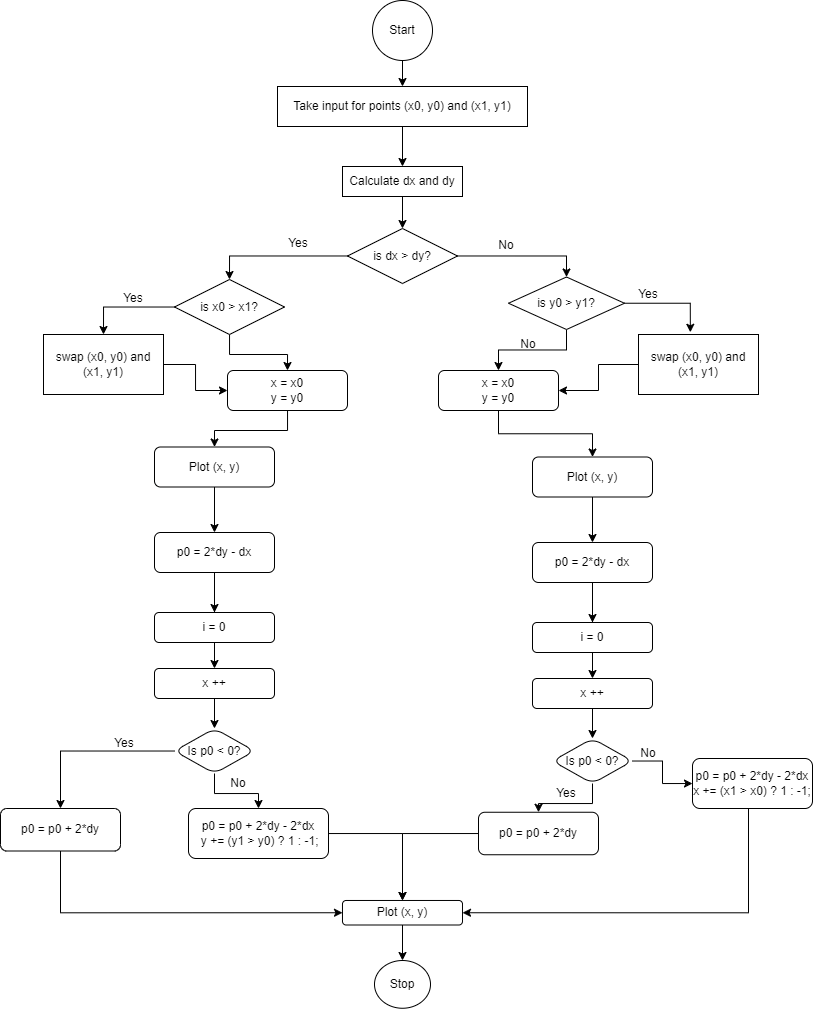
\includegraphics[width=0.7\textwidth]{flowchart.png}
\end{center}

\section*{SAMPLE I/O}
\textbf{Input:}
\begin{verbatim}
Enter the coordinates of the first point (x_start, y_start): -50 -50
Enter the coordinates of the second point (x_end, y_end): 50 50
\end{verbatim}

\textbf{Output:}
A line is drawn from $(-50, -50)$ to $(50, 50)$ on a window with coordinate axes displayed.

\section*{DISCUSSIONS}
\begin{itemize}
    \item \textbf{Accuracy}: Bresenham's algorithm provides a highly accurate and visually appealing way to draw lines because it minimizes the error and ensures that the line is continuous.
    \item \textbf{Efficiency}: The algorithm is computationally efficient as it uses only integer arithmetic, which is faster than floating-point operations.
    \item \textbf{Applications}: Beyond simple line drawing, Bresenham's algorithm is foundational in computer graphics and is used in rendering shapes, text, and other graphical elements.
\end{itemize}

\section*{CONCLUSION}
Bresenham's Line Drawing Algorithm is an essential algorithm in computer graphics for rendering straight lines with high efficiency and accuracy. The implementation using OpenGL effectively demonstrates the algorithm's capability to draw lines between any two points while also integrating the visualization of coordinate axes.

\section*{CODE LISTING}
\begin{lstlisting}[language=C]
#include <GL/glut.h>
#include <stdlib.h>
#include <stdio.h>
#include <math.h>

float x_start, y_start, x_end, y_end;

void init(void)
{
    glClearColor(0.0, 0.0, 0.0, 0.0);
    glMatrixMode(GL_PROJECTION);
    gluOrtho2D(-320.0, 320.0, -240.0, 240.0);
}

void setPixel(int x, int y)
{
    glBegin(GL_POINTS);
    glVertex2i(x, y);
    glEnd();
    glFlush();
}

void drawLineBresenham(float x_start, float y_start, float x_end, float y_end)
{
    int x0 = round(x_start);
    int y0 = round(y_start);
    int x1 = round(x_end);
    int y1 = round(y_end);
    int dx = abs(x1 - x0), sx = x0 < x1 ? 1 : -1;
    int dy = -abs(y1 - y0), sy = y0 < y1 ? 1 : -1;
    int err = dx + dy, e2;

    while (1)
    {
        setPixel(x0, y0);
        if (x0 == x1 && y0 == y1)
            break;
        e2 = 2 * err;
        if (e2 >= dy)
        {
            err += dy;
            x0 += sx;
        }
        if (e2 <= dx)
        {
            err += dx;
            y0 += sy;
        }
    }
}

void drawAxes(void)
{
    glColor3f(1.0, 1.0, 1.0);
    drawLineBresenham(-320, 0, 320, 0);
    drawLineBresenham(0, -240, 0, 240);
}

void display(void)
{
    glClear(GL_COLOR_BUFFER_BIT);
    drawAxes();
    glColor3f(0.0, 1.0, 1.0);
    drawLineBresenham(x_start, y_start, x_end, y_end);
    glFlush();
}

int main(int argc, char **argv)
{
    printf("Enter the coordinates of the first point (x_start, y_start): ");
    scanf("%f %f", &x_start, &y_start);
    printf("Enter the coordinates of the second point (x_end, y_end): ");
    scanf("%f %f", &x_end, &y_end);

    glutInit(&argc, argv);
    glutInitDisplayMode(GLUT_SINGLE | GLUT_RGB);
    glutInitWindowSize(640, 480);
    glutInitWindowPosition(100, 100);
    glutCreateWindow("Bresenham's Line Drawing Algorithm with Axes");
    init();
    glutDisplayFunc(display);
    glutMainLoop();

    return 0;
}
\end{lstlisting}

\end{document}
